\chapter{Illustrative Example}
\label{sec:example}

We next present a motivating example to describe the complexity of attacks on
DeFi protocols and our proposed approach to synthesize these attacks.
%providing a
%preemptive defense strategy to smart contracts developers to audit their
%contracts. 
%The example illustrates how our approach allows to sidestep the complexity of DeFi smart contracts which prevents the usage of existing verification techniques to adequately find attacks.  

\noindent \textbf{Background:} On October 26th 2020, an attacker exploited the
USDC and USDT vaults of Harvest Finance, causing a financial loss of about
$33.8$ million USD. In this chapter, we will focus on the attack on the USDC vault.
The attacker repeatedly executed the same attack vector 17 times targeting the USDC vault.
Fig.~\ref{fig:Harvest_USDC} summarizes the attack vector.
The attack vector contains a sequence of actions that interact with the following contracts:
\begin{itemize}
    \item \textbf{Uniswap:} Uniswap is an exchange protocol and it also offers flash loan services. The attacker borrows a large sum of USDC and USDT from Uniswap.

    \item \textbf{Curve:} Curve is an exchange protocol for stable coins like
        USDT, USDC, and DAI, whose market prices are close to one USD. It
        maintains pools of stable coins and users can interact with these pools
        to exchange one kind of stable coins to another. For example, Y Pool in
        Curve contains both USDC and USDT. Users can put USDC into the pool to
        exchange USDT out. The exchange rate fluctuates around one and it is
        determined by the current ratio of USDC and USDT in the pool. Note that
        Y pool automatically deposits USDT and USDC from users to \emph{Yearn},
        which is another DeFi protocol, and retrieves them back when the users
        withdraw. We omit this complication in this section for simplicity.

    \item \textbf{Harvest:} Harvest is an asset management protocol and the
        victim contract of this attack. Users can deposit USDC and USDT into
        Harvest and receive fUSDC and fUSDT tokens which users can later use to
        retrieve their deposit back. Harvest will invest the deposited USDC and
        USDT from users to other DeFi protocols to generate profit. Note that
        the exchange rate between fUSDC and USDC is also not fixed. It is
        determined by a closed source oracle contract, which ultimately
        also uses the pool ratio in Curve to calculate the rate.
\end{itemize}

%The attacker first repeatedly executed the same method that
%calls several methods in the DeFi protocol sequentially targeting the USDC
%vault. The attacker created $17$ transactions calling this method, which we
%will call \emph{the attack vector}. Afterwards, the attacker created $13$
%transactions calling another attack vector targeting the USDT vault. In the
%remainder of this section, we will focus on the first attack vector targeting
%the USDC vault.



\begin{figure}[t]
    \centering
    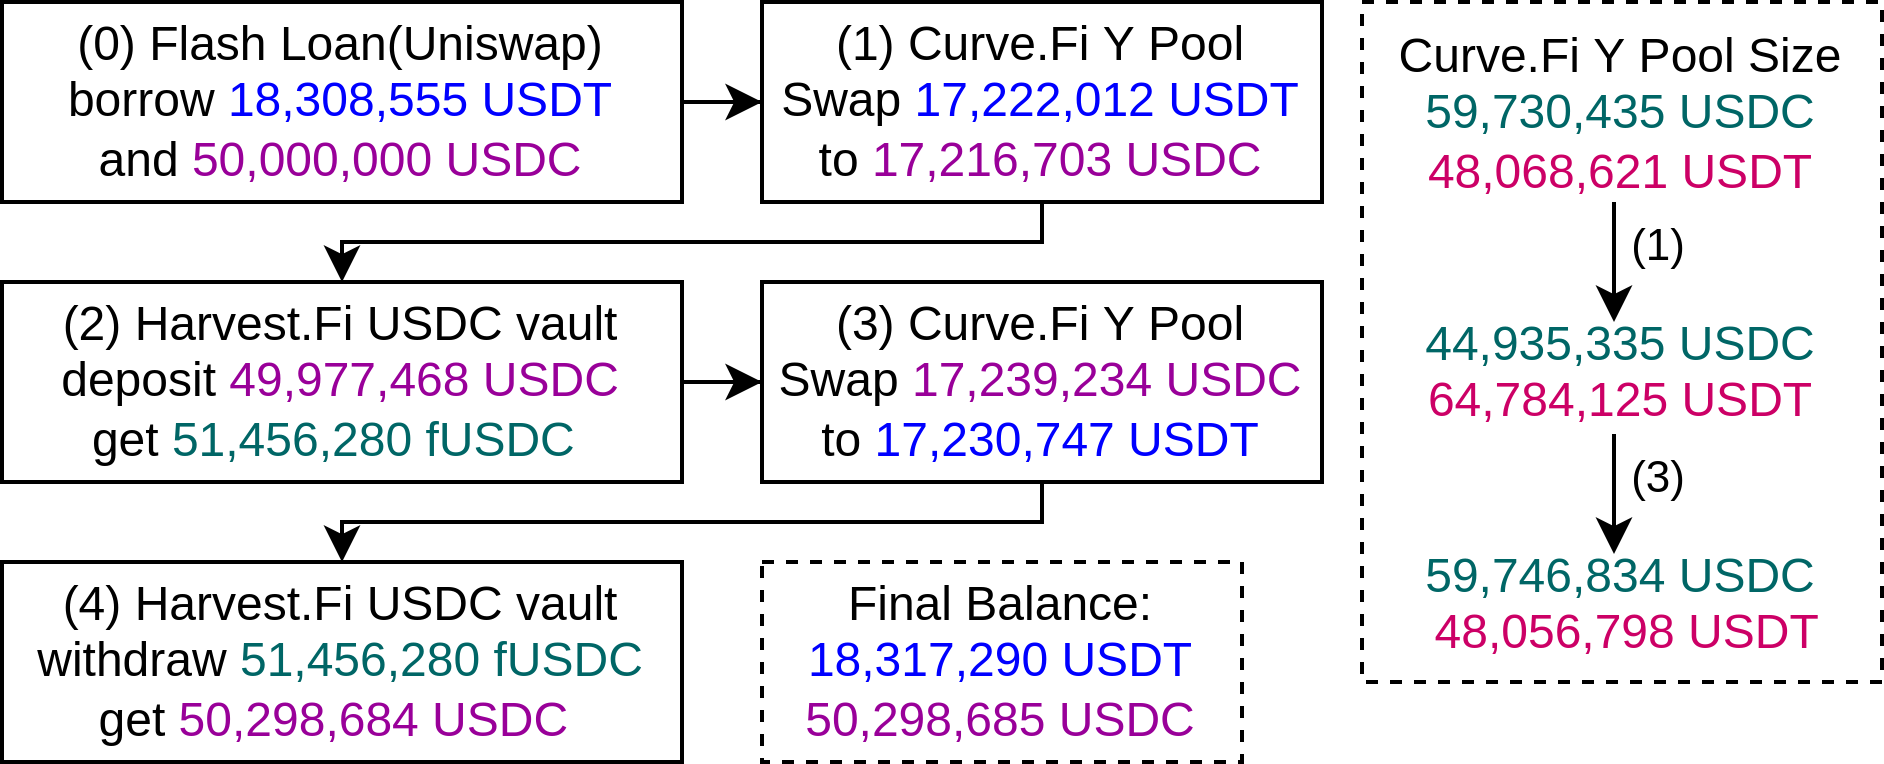
\includegraphics[width=\linewidth]{figures/Harvest_USDC3.png}
    \caption{Harvest USDC vault price manipulation attack.}
    \label{fig:Harvest_USDC}
\end{figure}

\noindent \textbf{Attack Actions:} The attack vector shown in
Fig.~\ref{fig:Harvest_USDC} first flash loaned $18.3$M USDT and $50$M USDC,
then called $4$ methods (actions) to exploit the design flaw in Harvest. The
first action, action $1$, consists of swapping USDT for USDC in Curve. It
transfers $17,222,012$ USDT to \emph{Curve.Fi Y Pool} and receives $17,216,703$
USDC back from Curve.
%The pool consumes yUSDC to withdraw $17,216,703$ USDC from \emph{Yearn USDC
%Vault} and transfers the amount to the attacker. 
Action $1$ reduces the estimated value of USDT based on the ratio in Y pool as
the amounts of USDT in Y Pool considerably increases. This in turn reduces
Harvest Finance's evaluation of its invested assets. Action $2$ deposits
$49,977,468$ USDC into \emph{Harvest Finance USDC vault} and due to the reduced
evaluation of the invested underlying assets, the attacker receives
$51,456,280$ fUSDC back, which is abnormally large. Similar to action $1$,
action $3$ then swaps $17,239,234$ USDC back to $17,230,747$ USDT via
\emph{Curve.Fi Y Pool}, which normalized the manipulated USDT/USDC rate in the
pool. It also brings Harvest Finance's evaluation of its invested underlying
asset back to normal. Finally, action $4$ withdraws $50,298,684$ USDC (using
$51,456,280$ fUSDC) from \emph{Harvest Finance USDC vault}. Assuming $1$ USDC
$= 1$ USDT $= 1$ USD, the profit of the above attack vector is $307,420$ USD. 

This attack is a typical case of oracle manipulation. The exploiter manipulated
the USDT/USDC rate in \emph{Curve.Fi Y Pool} by swapping a large amount between
USDC and USDT back and forth, which caused Harvest Finance protocol to
incorrectly evaluate the value of its asset, leaving large arbitrage space for
the exploiter. The actions sequence and particularly the parameters are
carefully chosen by the attacker to yield best profit. There are multiple
challenges {\name} faces to synthesize this attack.
%smart contracts developers to anticipate such attacks and to find the attacks
%vectors and their parameters to preemptively address them. 


\section{Challenges}

We now use the above attack as an example to illustrate the challenges. 

\noindent \textbf{Challenge 1 - Sophisticated Interactions:} The attack
involves several smart contracts that interact with each other and with
other contracts outside the attack vector. The state changes in one contract
influence the behavior of other contracts. For instance, actions $1$ and $3$
only change the states of \emph{Curve.Fi Y Pool}, but Harvest in actions $2$
and $4$ utilizes the states of \emph{Curve.Fi Y Pool} to calculate the amount to
deposit and withdraw.
%, their behaviors are influenced by actions $1$ and $3$. 
This makes the synthesis problem of finding an attack vector more complicated
as the effect of an action depends on its predecessor actions thus actions
cannot be treated separately.

\noindent \textbf{Challenge 2 - Close Source:} Some external smart contracts
that a DeFi protocol interacts with are not \emph{open-source}. For instance,
the source code of the external smart contract
\emph{PriceConverter}\footnote{Ethereum address:
0xfca4416d9def20ac5b6da8b8b322b6559770efbf} of Harvest Finance protocol is not
available on Etherscan~\cite{etherscan}, and it is called by actions $2$ and
$4$ to determine the exchange rate between fUSDC and USDC.
This impedes the complete understanding of the DeFi protocol implementation and
to reason about its correctness to anticipate attacks vectors.

\noindent \textbf{Challenge 3 - Mathematical Complexity:} DeFi contracts use
mathematical models that are too complex to reason about. For instance, actions
$2$ and $4$ swap an amount of token $i$ to token $j$, while maintaining the
following \emph{StableSwap invariant}~\cite{egorov2019stableswap}: 
$$A\cdot n^n\sum_i x_i  + D = A \cdot n^n \cdot D + \frac{D^{n+1}}{n^n \prod_{i}{x_i}}$$
where $A$ is a constant, $n$ is the number of the different types of tokens in
the pool ($4$ for \emph{Curve.Fi Y Pool}), $x_i$ is the liquidity of token $i$,
$D$ is the total amount of tokens when they have an equal price. Obviously
there does not exist a closed-form solution for $D$ as it requires finding
roots of a \emph{quintic equation}. Instead, in the actual smart contract
implementation, $D$ is calculated iteratively to a solution that maintains the
invariant.

%, using the liquidities before calling the function(see Figure~\ref{fig:new_get_D}). This kind of complex underlying mathematical models makes it hard to understand the exact execution results. 

% Next $x_i$ is increased subject to $dx$. Then, using the known $D$ and the updated $x_i$, the new $x_j$ is again calculated iteratively until the above invariant is satisfied again. The related source code is shown in Figures~\ref{fig:get_y} and~\ref{fig:get_D} in Appendix. 



% \begin{description}
%     \item[Preparation] flash loan of 18.3M USDT and 50M USDC.\footnote{This step is same for all attack vectors in this Section, and omitted later for brevity.}
%     \item[Action 1] \codeword{exchange_underlying(1, 2, 10554172e6, 0)} \footnote{Solidity supports scientific notations. The literal $MeE$ is equivalent to $M * 10^E$.} 
%     \item[Action 2] \codeword{deposit(49972546e6)} 
%     \item[Action 3] \codeword{exchange_underlying(2, 1, 10564726e6, 0)} 
%     \item[Action 4] \codeword{withdraw(51543726e6)} 
% \end{description}


% The function $exchange\_underlying$ requires four parameters, the two first parameters identify the token to swap ($1$ for USDC and $2$ for USDT), the third parameter specifies the quantity to swap, and the last parameter specifies the minimal quantity expected to receive from the swapping(neglect as it does not influence behaviors). 




\section{Failure of Symbolic Execution}
%\noindent \textbf{Symbolic Execution:} 
To demonstrate the complexity of DeFi protocols, we run an experiment with
Manticore~\cite{mossberg2019manticore}, a symbolic execution tool for smart
contracts, to execute the function \emph{get\_D}, for computing \emph{D} as
shown in Fig.~\ref{fig:new_get_D}, with symbolic inputs and explore all
possible reachable states. Manticore fails and throws a solver-related
exception together with an \emph{out of memory} error. We then simplified
\emph{get\_D} by removing the outer \emph{for} loop and bounding the length of
\emph{xp} to $2$, Manticore still fails and throws the same error. 
%The standard approach to search for such exploits is to use symbolic execution~\cite{king1976symbolic} to explore state space of related programs and check whether pre-defined invariants can be violated ~\cite{mossberg2019manticore,feng2019precise,mythril, luu2016making, cadar2008klee}.
%However, due to the complexity of DeFi protocols, it is difficult for these symbolic execution based tools to reach all program states, which might extract an overly complex symbolic constraints and easily exhaust the underlying solvers to time out.
%For instance, to test the applicability of symbolic execution, we tried to symbolically execute an internal function $get\_D$(Figure ~\ref{fig:new_get_D}), which is called inside the function $exchange\_underlying$. 
%We use Manticore~\cite{mossberg2019manticore} to execute $get\_D$ with symbolic inputs and explore all possible states it can reach. 
%Manticore fails and throws a solver-related exception together with an \emph{out of memory} error. 
%We then simplify $get\_D$ by removing the $for$ loop and bounding the length of $xp$ to 2, Manticore still fails and throws the same error. 


\input{solidity-highlighting.tex}
\begin{figure}[t]
    \centering
    \begin{minipage}[h]{0.9\linewidth}
    \lstinputlisting{codes/new_get_D.sol}
    \end{minipage}
    \vspace{-3mm}
    \caption{\emph{get\_D} method to compute \emph{D}.}
 \vspace{-5mm}
\label{fig:new_get_D}
\end{figure}



\section{Usage of \name{}}
We propose \name{}, a framework to tackle the problem of synthesizing attack vectors for given DeFi protocols. 
\name{} synthesizes attack vectors using counterexample-driven approximation to model the behavior of the protocols. 
\name{} solves the first challenge by computing a state transition function for
each state element an action alters. The approximation used by \name{} solves
the second and third challenges since we no longer need the actual
implementation. 

We next show how to use {\name} to synthesize the Harvest USDC vault attack. 

\noindent \textbf{Identify Candidate Actions: }
\name{} first takes a set of actions as inputs from users, i.e., methods inside smart contracts. 
For instance, a set of candidate actions for the Harvest USDC attack can be as
follows: \codeword{exchange(USDT, USDC, v)}, \codeword{deposit(v)},
\codeword{exchange(USDC, USDT, v)}, and \codeword{withdraw(v)}. The first two
input arguments to \codeword{exchange} specify the token types to be swapped.
The third argument specifies the quantity to swap\footnote{Note that in the
implementation the actual name of the \codeword{exchange} method is
\codeword{exchange\_underlying}, $1$ and $2$ are used to identify the tokens
USDC and USDT, respectively, and the method has a fourth argument to specify
the minimal quantity expected to receive from the swapping.}.


\noindent \textbf{Identify Input/Output States and Tokens: }
Our approach then requires users to provide action specifications(Figure~\ref{table:prepost_harvest_usdc}), which is a set of prestates, poststates, input token(s) and output token(s). Our approach utilizes these states to infer approximated state transition functions for each action candidates. This allows to abstract internal interactions among DeFi protocols, and eliminates the requirements of open source smart contracts. 

We use $\stateof{1}$, $\stateof{2}$, $\stateof{3}$, $\stateof{4}$, and $\stateof{5}$ to represent the key states in the Harvest USDC attack 
and in Table~\ref{table:prepost_harvest_usdc} we list the set the of prestates and prostates for each action. Note all the states can be read by public read-only functions inside relevant smart contracts. States $\stateof{1}$ and $\stateof{2}$ represent USDC and USDT liquidities in the Curve.Fi Y Pool. States $\stateof{3}$, $\stateof{4}$, and $\stateof{5}$ represent the underlying balance of the vault, the invested balance of the vault, and fUSDC total supply, respectively. 
Actions \codeword{exchange(USDT,USDC,-)} and \codeword{exchange(USDC,USDT,-)} change the liquidities of USDC($\stateof{1}$) and USDT($\stateof{2}$). This also results in Harvest Finance changing its evaluation of the value of its invested balance ($\stateof{4}$). Action \codeword{deposit(-)} deposits USDC to the vault(changes $\stateof{3}$), and the vault mints(changes $\stateof{5}$) and sends back fUSDC in return. Action \codeword{withdraw(-)} returns fUSDC back to the vault, burns them(changes $\stateof{5}$) and withdraws USDC from the vault(changes $\stateof{3}$). The exchange rate of fUSDC and USDC within \codeword{deposit} and \codeword{withdraw} are dependent on Harvest Finance protocol's balance in the vault ($\stateof{3}$), the invested Balance ($\stateof{4}$), and fUSDC total supply ($\stateof{5}$).

\input{solidity-highlighting.tex}
\begin{figure}[t]
    \centering
    \begin{minipage}[h]{1.0\linewidth}
    \lstinputlisting{codes/new_vault.sol}
    \end{minipage}
    \vspace{-3mm}
    \caption{The Vault \codeword{deposit} and \codeword{withdraw} methods.}
 \label{fig:depositwithdraw}
 \vspace{-5mm}
\end{figure}


\begin{table}[!h]
    \caption{Actions in Harvest USDC Vault attack}
    
    Notes: \textbf{IDP} and \textbf{TDP} represent the initial and total number of datapoints.
    \label{table:prepost_harvest_usdc}
    \centering
    \begin{tabular}{|l|l|l|l|l|l|}
    \hline
    Action    & Prestates  & Poststates & IDP & TDP & TDP\\ 
              &            &  &  & Poly & Inter \\\hline
    exchange  & $\stateof{1}$, $\stateof{2}$, $\stateof{4}$  & $\stateof{1}'$, $\stateof{2}'$, $\stateof{4}'$  & 2000 & 2238 & 2792      \\ 
    (USDT, USDC, v) &   &  &  &  &  \\\hline
    exchange  & $\stateof{1}$, $\stateof{2}$, $\stateof{4}$   & $\stateof{1}'$, $\stateof{2}'$, $\stateof{4}'$    & 2000 & 2148 & 2888     \\ 
    (USDC, USDT, v) &  &  &  &  &      \\ \hline
    deposit(v)  & $\stateof{3}$, $\stateof{4}$, $\stateof{5}$ & $\stateof{3}'$, $\stateof{5}'$    & 2000 & 2162 & 2358   \\ \hline
    withdraw(v)  & $\stateof{3}$, $\stateof{4}$, $\stateof{5}$ & $\stateof{3}'$, $\stateof{5}'$   & 2000 & 2364 & 2876      \\ \hline
    \end{tabular}
\end{table}


\noindent \textbf{Capture Initial Approximation: } In our approach, for each action in Table~\ref{table:prepost_harvest_usdc} {\name} infers a state transition function that accepts the action's input parameters and transforms the prestates to poststates and returns the action's output parameters. For instance, the actions corresponding to \codeword{exchange} change the states $\stateof{1}$, $\stateof{2}$, and $\stateof{4}$. Our approach infers expressions relating the poststates $\stateof{1}'$, $\stateof{2}'$, and $\stateof{4}'$ and the outputted amount of USDC to the prestates $\stateof{1}$, $\stateof{2}$, and $\stateof{4}$ and the input parameter of \codeword{exchange}. 
Similarly, the actions associated with \codeword{deposit} and \codeword{withdraw} alter the states $\stateof{3}$ and $\stateof{5}$ of Harvest Finance.

{\name} first collects a set of data points where each data point is defined as an \textit{input-output} pair, where the \textit{input} is the action's prestates and its input parameters, and the \textit{output} is its poststates and the outputted values. {\name} also executes dependent actions beforehand to reach a wide range of data points. 

For instance, for \codeword{exchange(USDC,USDT,-)}, notice its prestates can be altered by itself or another action \codeword{exchange(USDT,USDC,-)}. Therefore, {\name} executes \codeword{exchange(USDC,USDT,-)} or \codeword{exchange(USDT,USDC,-)} before collecting data points for \codeword{exchange(USDC,USDT,-)}. The parameters are all sampled from given ranges(e.g., $(0, u)$ where $u$ is an upper limit of the parameters given by the user). Then, we use these data points to find the best approximated state transition functions. 

We consider two methods to solve the above multivariate approximation problem: linear regression based polynomial features method and nearest-neighbor interpolation method. In the first method, we generate a feature matrix consisting of all polynomial combinations of the features with degree less than or equal to $n$. Then, we use linear regression to find the optimal coefficients and degree for the polynomial function $f$. In the second method, we build a nearest-$N$-dimensional interpolator based on the input-output pairs. 


\noindent \textbf{Enumerate and Filter Action Sequence: } After capturing an
initial approximation of state transition functions, {\name} leverages an
enumeration-based top-down algorithm to synthesize different action sequences. 
{\name} uses several pruning heuristics applied to filter
unpromising sequences, e.g., sequences with two adjacent actions calling the
same method.
For each enumerated action sequence, {\name} uses the approximated state
transition functions to construct an optimization problem, consisting of an
objective function that represents profit and constraints. {\name} then applies
an off-the-shelf optimizer to obtain a list of parameters that maximize the
profit estimated using approximated transition functions. 
{\name} also prunes away action sequences that the optimizer cannot
find any parameters which yield an estimated positive profit.

%\subsubsection{Verify Synthesized Results}
%its actual profit its estimated profit, {\name}
%considers it as correct and includes it in the final return output if the
%profit is positive. If not, {\name} reports it as a counterexample, which
%indicates inaccuracy of our approximated transition functions. 

% due to the limited state space explored during the initial round of data collection.

%\subsubsection{Counterexample Driven Refinement}
% In particular, when tested on a new sequence of actions that was not covered in initial round, our approximations might return inaccurate results if no data points were collected near the prestates reached when executing the sequence of actions.
\noindent \textbf{Counterexample Driven Refinement: } After getting a list of parameters that maximize the estimated profit of one
action sequence, {\name} verifies synthesized attack vectors by actually
executing them in the private blockchain and checks their actual profit. For an
attack vector, if the difference margin between the actual profit and the
estimated profit is greater than $5\%$, {\name} reports it as a counterexample,
which indicates inaccuracy of our approximated transition functions. To correct
this inaccuracy, {\name} employs a new \textit{counterexample-driven
approximation refinement} technique. {\name} uses the reported counterexamples
to collect new data points to refine the approximations. The new approximations
are used to search for parameters that maximize the profit over action
sequences.

%The above process is repeated iteratively. 
\noindent \textbf{Synthesized Attack:} In the Harvest USDC example, {\name}
successfully found the following attack vector that yields an adjusted profit
of $110051$ USD using the interpolation technique with the counterexample
driven refinement loop. \\ 

$\codeword{exchange(USDT, USDC, 15192122)} \cdot
\codeword{deposit(45105321)}\ \cdot \codeword{exchange(USDC, USDT, 11995404)} \cdot
\codeword{withdraw(46198643)}$\\

%Note that our approach is able to synthesize a new attack vector with different action sequence from the Harvest Finance USDC attack vector in history.
Note that the synthesized attack vector has the same action sequence and
similar parameters as used by the exploiter in history. The last three columns
of Table~\ref{table:prepost_harvest_usdc} list the number of data points
collected initially (without counterexamples) and the total number of data
points for both polynomial and interpolation, respectively.  Such profitable attack vectors are direct proofs of the vulnerabilities inside Harvest Finance protocols, as they reveal a way to cause financial loss to relevant DeFi smart contracts. 

\begin{comment}
\begin{table}[t]
\caption{Number of Data Points for Harvest USDC(\textbf{Start} represents the total number of data points after initial pass of data collection. \textbf{End(X)} represents that at the end of synthesis using \textbf{X} method)}
\label{table:datapoints_Harvest_USDC}
\centering
\scriptsize
\begin{tabular}{|l|l|l|l|}
\hline
Action & Start & End(Polynomial) & End(Interpolation) \\ \hline
exchange(2, 1, -) & 2000 & 2238 & 2792 \\ \hline
exchange(1, 2, -) & 2000 & 2148 & 2888 \\ \hline
deposit(-) & 2000 & 2162 & 2358 \\ \hline
withdraw(-) & 2000 & 2364 & 2876 \\ \hline
\end{tabular}
\end{table}
\end{comment}
\begin{comment}


\subsubsection{Synthesize Action Sequence and Optimize}
After capturing an initial approximation of state transition functions, {\name} leverages an enumeration-based top-down algorithm to synthesize different action sequences, with several pruning heuristics applied to eliminate infeasible ones(details in Section ~\ref{sec:isfeasible}). For each feasible action sequence, using the approximated state transition functions, {\name} automatically constructs an optimization framework(details in Section ~\ref{sec:opframe}), consisting of an objective function(which represents profit) and constraints. Then {\name} applies an off-the-shelf optimizer to solve the optimization framework, and get a list of parameters that maximize the profit estimated using approximated transition functions. 

\subsubsection{Verify Synthesized Results}
After getting a list of parameters that maximize the estimated profit of one action sequence, {\name} verifies synthesized attack vectors by executing them in a forked environment and checking their actual profit. For an attack vector, if its actual profit matches its estimated profit, {\name} considers it as correct and include it in the final return output. If not, {\name} reports it as a counterexample, which indicates inaccuracy of our approximated transition functions. 

% due to the limited state space explored during the initial round of data collection.

\subsubsection{Counterexample Driven Refinement}
% In particular, when tested on a new sequence of actions that was not covered in initial round, our approximations might return inaccurate results if no data points were collected near the prestates reached when executing the sequence of actions.
To overcome the above inaccuracy we introduce a novel \textit{counterexample-driven approximation refinement} technique. In brief, these counterexamples reported by {\name} are utilized to collect new data points and refine approximations. And the modified approximations are used again search for action sequences and parameters that maximize the profit. This process is repeated iteratively. In the Harvest USDC example, the number of data points collected in the beginning and in the end is listed in Table~\ref{table:datapoints_Harvest_USDC}. 

Using our approach, we successfully find the following attack vector that yields an adjusted profit of 110051 USD. 
\begin{description}
    \item[Action 1: \codeword{exchange(2, 1, 15192122e6)}]
    \item[Action 2: \codeword{deposit(45105321e6)}]
    \item[Action 3: \codeword{exchange(1, 2, 11995404e6)}] 
    \item[Action 4: \codeword{withdraw(46198643e6)}] 
\end{description}
%Note that our approach is able to synthesize a new attack vector with different action sequence from the Harvest Finance USDC attack vector in history.
Note the synthesized attack vector has the same action sequence and similar parameters  as used by the exploiter in history. Such profitable attack vectors are direct proofs of the vulnerabilities inside Harvest Finance protocols, as they reveal a way to cause financial loss to relevant DeFi smart contracts. 


\begin{table}[t]
\caption{Number of Data Points for Harvest USDC(\textbf{Start} represents the total number of data points after initial pass of data collection. \textbf{End(X)} represents that at the end of synthesis using \textbf{X} method)}
\label{table:datapoints_Harvest_USDC}
\centering
\scriptsize

\begin{tabular}{|l|l|l|l|}
\hline
Action & Start & End(Polynomial) & End(Interpolation) \\ \hline
exchange(2, 1, -) & 2000 & 2238 & 2792 \\ \hline
exchange(1, 2, -) & 2000 & 2148 & 2888 \\ \hline
deposit(-) & 2000 & 2162 & 2358 \\ \hline
withdraw(-) & 2000 & 2364 & 2876 \\ \hline
\end{tabular}
\end{table}

\end{comment}

